\documentclass{article}

\usepackage{graphicx}
\usepackage{tikz}
\usepackage{tikzsymbols}
\usetikzlibrary{calc,patterns,shapes.geometric}
\pagestyle{empty}
\usepackage[margin=0pt]{geometry}
\geometry{papersize={14in,12in}}

\def\centerarc[#1](#2)(#3:#4:#5){\draw[#1] ($(#2)+({#5*cos(#3)},{#5*sin(#3)})$) arc (#3:#4:#5);}

\begin{document}
	\begin{figure}
		\centering
		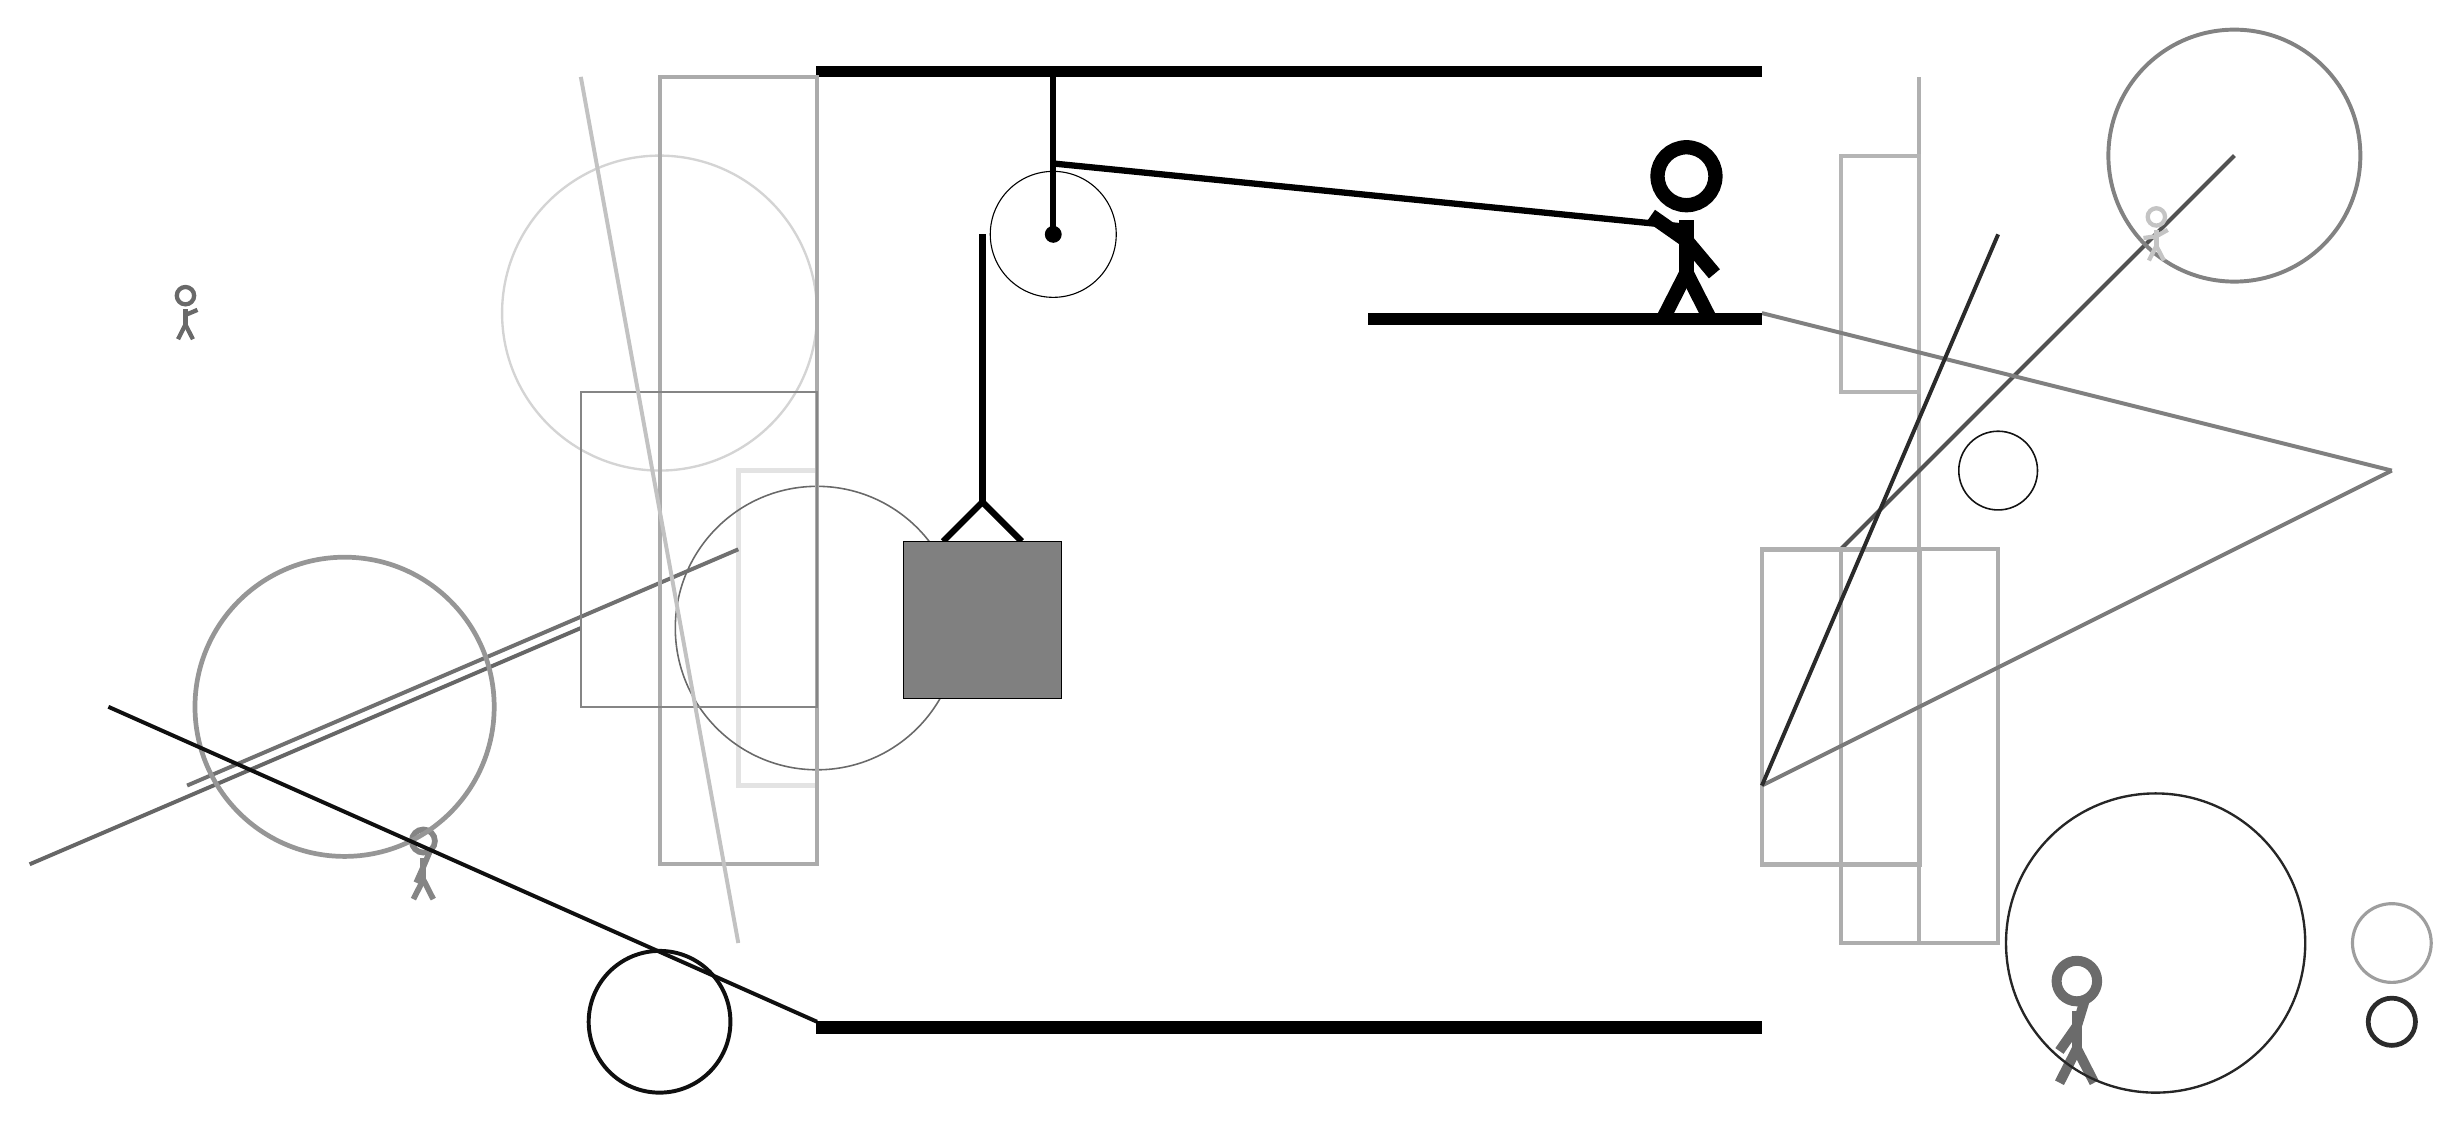
\begin{tikzpicture}
			%%%%% START %%%%%
			
			\draw[fill=black] (-2, 9) rectangle (10, 9.125);
			
			\node[line width=0.2mm, color=black!58] at (14, -3) {\Strichmaxerl[7][55][73]};
			
			\draw[line width=0.5mm, color=black!44](-5, 2) -- (-5, 2);
			\draw[line width=0.6mm, color=black!11] (-2, 0) rectangle (-3, 4);
			\draw[line width=0.5mm, color=black!60](-5, 2) -- (-12, -1);
			\draw [line width=0.2mm, color=black!93](13, 4) circle (0.5);
			
			\draw [line width=0.5mm, color=black!30](17, 1) circle (0.0);
			\draw [line width=0.5mm, color=black!94](-4, -3) circle (0.9);
			
			\draw[line width=0.5mm, color=black!31](12, -2) -- (12, 9);
			\draw [line width=0.2mm, color=black!59](-2, 2) circle (1.8);
			\draw[line width=0.5mm, color=black!32] (11, -2) rectangle (13, 3);
			
			\draw [line width=0.3mm, color=black!85](15, -2) circle (1.9);
			
			\draw[line width=0.5mm, color=black!56](-3, 3) -- (-10, 0);
			\draw [line width=0.4mm, color=black!38](18, -2) circle (0.5);
			
			\draw[line width=0.5mm, color=black!29] (11, 8) rectangle (12, 5);
			\node[line width=0.5mm, color=black!48] at (-7, -1) {\Strichmaxerl[4][66][67]};
			\draw[line width=0.5mm, color=black!68](11, 3) -- (16, 8);
			
			\draw [line width=0.3mm, color=black!17](-4, 6) circle (2.0);
			
			\node[line width=0.2mm, color=black!59] at (-10, 6) {\Strichmaxerl[3][89][23]};
			\draw [line width=0.5mm, color=black!49](16, 8) circle (1.6);
			\draw [line width=0.6mm, color=black!41](-8, 1) circle (1.9);
			\draw [line width=0.6mm, color=black!83](18, -3) circle (0.3);
			
			\draw[line width=0.5mm, color=black!33] (-2, -1) rectangle (-4, 9);
			\draw[line width=0.5mm, color=black!50](10, 6) -- (18, 4);
			\draw[line width=0.6mm, color=black!31] (10, -1) rectangle (12, 3);
			\draw[line width=0.2mm, color=black!48] (-2, 5) rectangle (-5, 1);
			
			\draw[line width=0.5mm, color=black!52](10, 0) -- (18, 4);
			\node[line width=0.7mm, color=black!23] at (15, 7) {\Strichmaxerl[3][8][29]};
			\draw[line width=0.5mm, color=black!83](13, 7) -- (10, 0);
			
			\draw[line width=0.5mm, color=black!94](-2, -3) -- (-11, 1);
			\draw[line width=0.5mm, color=black!24](-3, -2) -- (-5, 9);
			
			\draw (1, 7) circle (0.8);
			\draw[fill=black] (1, 7) circle (0.1);
			\draw[line width=0.8mm] (1, 9) -- (1, 7);
			
			\draw[line width=0.8mm](-0.4, 3.1) --  (0.1, 3.6) -- (0.6, 3.1);
			\draw[fill=black!50] (-0.9, 3.1) rectangle (1.1, 1.1);
			
			\draw[line width=0.8mm](0.1, 7) -- (0.1, 3.6);
			\centerarc[line width=0.8mm](1, 7)(90:180:0.9)
			\draw[line width=0.8mm](1, 7.9) -- (9, 7.1);
			
			\node at (9, 7) {\Strichmaxerl[10][-35][-50]};
			\draw[fill=black] (5, 6) rectangle (10, 5.85);
			
			\draw[fill=black] (-2, -3) rectangle (10, -3.15);
			
			%%%%% END %%%%%
		\end{tikzpicture}
	\end{figure}	
\end{document}